\chapter{Interactive Demo Application}
We designed and implemented an interactive demo application\footnote{\url{http://switch.blenderdemo.com:8501/}} hosted on an AWS Cloud server to demonstrate our framing analysis functionalities. The demo application is based on Streamlit\footnote{\url{https://streamlit.io/}}. In the following sections, we elaborate on two functionalities of the demo application: 1) Text generation controlled by user-specified left-right stance position in \refsec{demo-generation}, and 2) Left-right stance categorization given text input in \refsec{demo-detection}.


\section{Stance-guided Generation}
\label{demo-generation}
A screenshot of the interface for Stance-guided Generation is shown in \reffig{fig:demo-generation}. A continuous slide bar controls the left-right position of text generation, and the user can specify the random seed and the max/min generation length for more generation control. The user can then input prefix text for the model to continue writing. After the ``Generate!'' button is clicked, the generated text will be displayed.


\begin{figure}[ht]
    \centering
    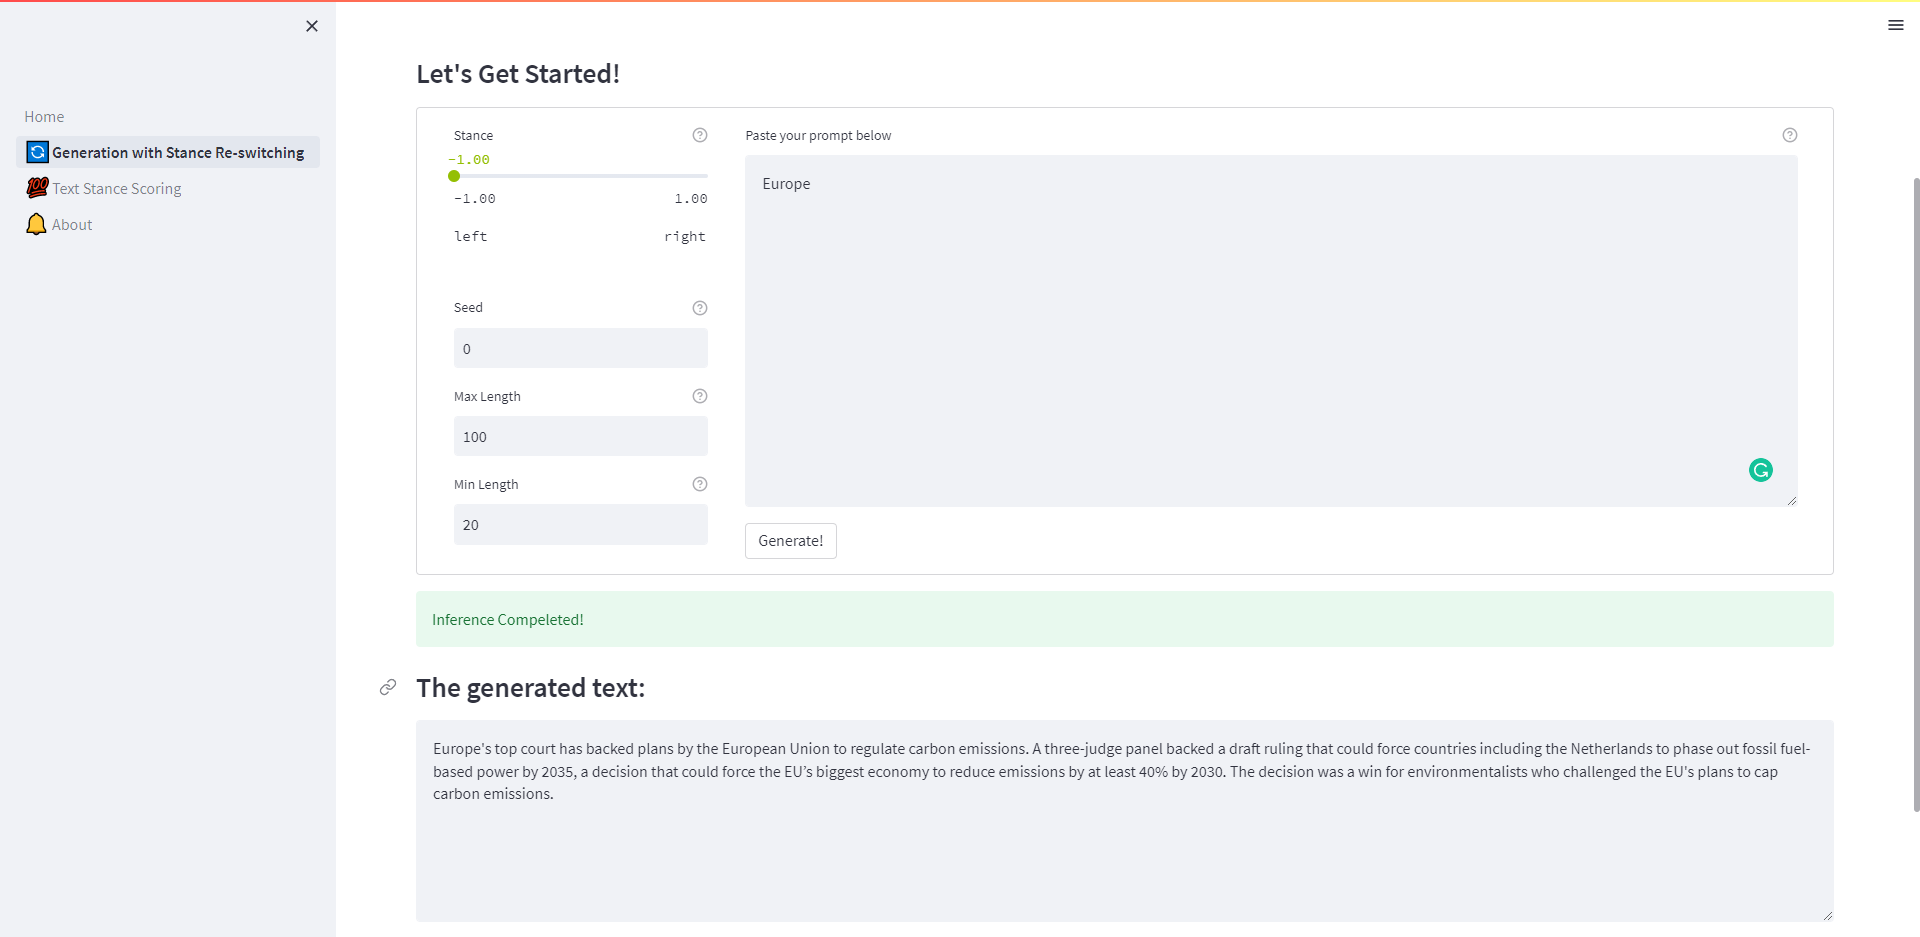
\includegraphics[width=\textwidth]{img/demo-generation}
    \caption{The interface of the Stance-guided Generation functionality.}
    \label{fig:demo-generation}
\end{figure}


\section{Stance Categorization}
\label{demo-detection}
A screenshot of the interface for Stance Categorization is shown in \reffig{fig:demo-detection}. An input box allows the user to put in the text to be analyzed. After clicking on the ``Analyze!'' button, two results will be output and displayed: 1) distribution of the probability across all 7 different stance categories, in the form of a histogram chart, and 2) a list-out of text spans that serve as evidence for the stance categorization and their evidence scores.


\begin{figure}[ht]
    \centering
    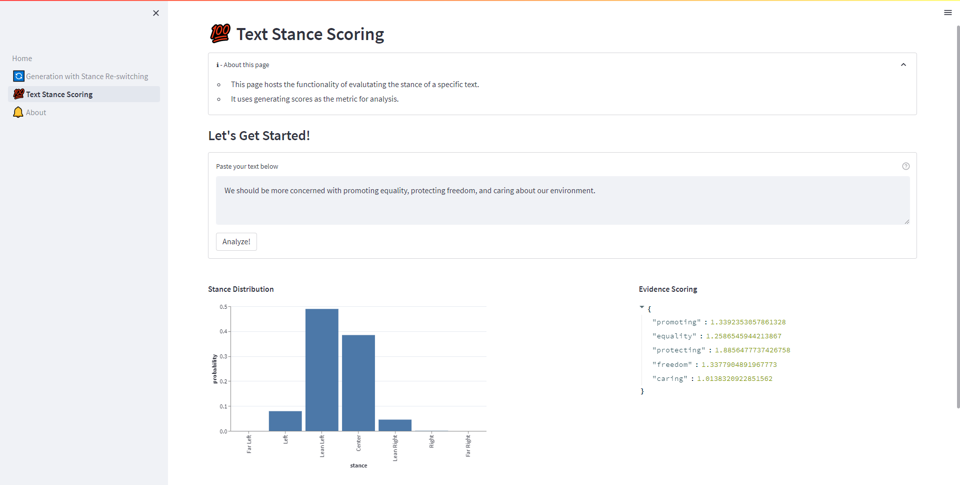
\includegraphics[width=\textwidth]{img/demo-detection}
    \caption{The interface of the Stance Categorization functionality.}
    \label{fig:demo-detection}
\end{figure}